% Options for packages loaded elsewhere
\PassOptionsToPackage{unicode}{hyperref}
\PassOptionsToPackage{hyphens}{url}
%
\documentclass[
  12pt,
  ignorenonframetext,
  aspectratio=169,
]{beamer}
\usepackage{pgfpages}
\setbeamertemplate{caption}[numbered]
\setbeamertemplate{caption label separator}{: }
\setbeamercolor{caption name}{fg=normal text.fg}
\beamertemplatenavigationsymbolsempty
% Prevent slide breaks in the middle of a paragraph
\widowpenalties 1 10000
\raggedbottom
\setbeamertemplate{part page}{
  \centering
  \begin{beamercolorbox}[sep=16pt,center]{part title}
    \usebeamerfont{part title}\insertpart\par
  \end{beamercolorbox}
}
\setbeamertemplate{section page}{
  \centering
  \begin{beamercolorbox}[sep=12pt,center]{part title}
    \usebeamerfont{section title}\insertsection\par
  \end{beamercolorbox}
}
\setbeamertemplate{subsection page}{
  \centering
  \begin{beamercolorbox}[sep=8pt,center]{part title}
    \usebeamerfont{subsection title}\insertsubsection\par
  \end{beamercolorbox}
}
\AtBeginPart{
  \frame{\partpage}
}
\AtBeginSection{
  \ifbibliography
  \else
    \frame{\sectionpage}
  \fi
}
\AtBeginSubsection{
  \frame{\subsectionpage}
}
\usepackage{lmodern}
\usepackage{amssymb,amsmath}
\usepackage{ifxetex,ifluatex}
\ifnum 0\ifxetex 1\fi\ifluatex 1\fi=0 % if pdftex
  \usepackage[T1]{fontenc}
  \usepackage[utf8]{inputenc}
  \usepackage{textcomp} % provide euro and other symbols
\else % if luatex or xetex
  \ifxetex
    \usepackage{mathspec}
  \else
    \usepackage{unicode-math}
  \fi
  \defaultfontfeatures{Scale=MatchLowercase}
  \defaultfontfeatures[\rmfamily]{Ligatures=TeX,Scale=1}
\fi
\usetheme[]{Dresden}
\usecolortheme{dolphin}
\usefonttheme{structurebold}
% Use upquote if available, for straight quotes in verbatim environments
\IfFileExists{upquote.sty}{\usepackage{upquote}}{}
\IfFileExists{microtype.sty}{% use microtype if available
  \usepackage[]{microtype}
  \UseMicrotypeSet[protrusion]{basicmath} % disable protrusion for tt fonts
}{}
\makeatletter
\@ifundefined{KOMAClassName}{% if non-KOMA class
  \IfFileExists{parskip.sty}{%
    \usepackage{parskip}
  }{% else
    \setlength{\parindent}{0pt}
    \setlength{\parskip}{6pt plus 2pt minus 1pt}}
}{% if KOMA class
  \KOMAoptions{parskip=half}}
\makeatother
\usepackage{xcolor}
\IfFileExists{xurl.sty}{\usepackage{xurl}}{} % add URL line breaks if available
\IfFileExists{bookmark.sty}{\usepackage{bookmark}}{\usepackage{hyperref}}
\hypersetup{
  pdftitle={Statistical Thinking in Biology Research},
  pdfauthor={Terry Neeman},
  hidelinks,
  pdfcreator={LaTeX via pandoc}}
\urlstyle{same} % disable monospaced font for URLs
\newif\ifbibliography
\usepackage{color}
\usepackage{fancyvrb}
\newcommand{\VerbBar}{|}
\newcommand{\VERB}{\Verb[commandchars=\\\{\}]}
\DefineVerbatimEnvironment{Highlighting}{Verbatim}{commandchars=\\\{\}}
% Add ',fontsize=\small' for more characters per line
\usepackage{framed}
\definecolor{shadecolor}{RGB}{248,248,248}
\newenvironment{Shaded}{\begin{snugshade}}{\end{snugshade}}
\newcommand{\AlertTok}[1]{\textcolor[rgb]{0.94,0.16,0.16}{#1}}
\newcommand{\AnnotationTok}[1]{\textcolor[rgb]{0.56,0.35,0.01}{\textbf{\textit{#1}}}}
\newcommand{\AttributeTok}[1]{\textcolor[rgb]{0.77,0.63,0.00}{#1}}
\newcommand{\BaseNTok}[1]{\textcolor[rgb]{0.00,0.00,0.81}{#1}}
\newcommand{\BuiltInTok}[1]{#1}
\newcommand{\CharTok}[1]{\textcolor[rgb]{0.31,0.60,0.02}{#1}}
\newcommand{\CommentTok}[1]{\textcolor[rgb]{0.56,0.35,0.01}{\textit{#1}}}
\newcommand{\CommentVarTok}[1]{\textcolor[rgb]{0.56,0.35,0.01}{\textbf{\textit{#1}}}}
\newcommand{\ConstantTok}[1]{\textcolor[rgb]{0.00,0.00,0.00}{#1}}
\newcommand{\ControlFlowTok}[1]{\textcolor[rgb]{0.13,0.29,0.53}{\textbf{#1}}}
\newcommand{\DataTypeTok}[1]{\textcolor[rgb]{0.13,0.29,0.53}{#1}}
\newcommand{\DecValTok}[1]{\textcolor[rgb]{0.00,0.00,0.81}{#1}}
\newcommand{\DocumentationTok}[1]{\textcolor[rgb]{0.56,0.35,0.01}{\textbf{\textit{#1}}}}
\newcommand{\ErrorTok}[1]{\textcolor[rgb]{0.64,0.00,0.00}{\textbf{#1}}}
\newcommand{\ExtensionTok}[1]{#1}
\newcommand{\FloatTok}[1]{\textcolor[rgb]{0.00,0.00,0.81}{#1}}
\newcommand{\FunctionTok}[1]{\textcolor[rgb]{0.00,0.00,0.00}{#1}}
\newcommand{\ImportTok}[1]{#1}
\newcommand{\InformationTok}[1]{\textcolor[rgb]{0.56,0.35,0.01}{\textbf{\textit{#1}}}}
\newcommand{\KeywordTok}[1]{\textcolor[rgb]{0.13,0.29,0.53}{\textbf{#1}}}
\newcommand{\NormalTok}[1]{#1}
\newcommand{\OperatorTok}[1]{\textcolor[rgb]{0.81,0.36,0.00}{\textbf{#1}}}
\newcommand{\OtherTok}[1]{\textcolor[rgb]{0.56,0.35,0.01}{#1}}
\newcommand{\PreprocessorTok}[1]{\textcolor[rgb]{0.56,0.35,0.01}{\textit{#1}}}
\newcommand{\RegionMarkerTok}[1]{#1}
\newcommand{\SpecialCharTok}[1]{\textcolor[rgb]{0.00,0.00,0.00}{#1}}
\newcommand{\SpecialStringTok}[1]{\textcolor[rgb]{0.31,0.60,0.02}{#1}}
\newcommand{\StringTok}[1]{\textcolor[rgb]{0.31,0.60,0.02}{#1}}
\newcommand{\VariableTok}[1]{\textcolor[rgb]{0.00,0.00,0.00}{#1}}
\newcommand{\VerbatimStringTok}[1]{\textcolor[rgb]{0.31,0.60,0.02}{#1}}
\newcommand{\WarningTok}[1]{\textcolor[rgb]{0.56,0.35,0.01}{\textbf{\textit{#1}}}}
\setlength{\emergencystretch}{3em} % prevent overfull lines
\providecommand{\tightlist}{%
  \setlength{\itemsep}{0pt}\setlength{\parskip}{0pt}}
\setcounter{secnumdepth}{-\maxdimen} % remove section numbering
\usepackage{fancyvrb}

\title{Statistical Thinking in Biology Research}
\subtitle{Probability and Statistical Inference}
\author{Terry Neeman}
\date{30th July 2020}
\institute{Australian National University}

\begin{document}
\frame{\titlepage}

\begin{frame}{A few key ideas}
\protect\hypertarget{a-few-key-ideas}{}

\begin{itemize}
\tightlist
\item
  Probability: understanding possible outcomes under a set of ``rules''
\item
  Domain of probability: mathematics (``theoretical'', ``proof'')
\item
  Statistics: Given a set of outcomes, what can we \emph{infer} about
  the possible rules?
\item
  Domain of statistics: real world data (``pragmatic'', ``heuristic'')
\end{itemize}

\begin{block}{Probability and Statistics are two sides of the same
subject.}

\end{block}

\end{frame}

\begin{frame}{Probability: measures of uncertainty}
\protect\hypertarget{probability-measures-of-uncertainty}{}

\begin{itemize}
\tightlist
\item
  Sample space: space of possible outcomes
\item
  Distribution: relative frequencies (probabilities) of each outcome
\item
  Summaries of distributions: average (expected) outcome, variation
  around average
\end{itemize}

\end{frame}

\begin{frame}{Examples of common distributions in biological research}
\protect\hypertarget{examples-of-common-distributions-in-biological-research}{}

\begin{itemize}
\tightlist
\item
  Normal distribution

  \begin{itemize}
  \tightlist
  \item
    family of distributions
  \item
    defined by two parameters: mean and standard deviation (variance)
  \item
    many biological measures normally distributed, e.g.~height, weight
  \end{itemize}
\end{itemize}

\end{frame}

\begin{frame}[fragile]{Sample from a normal distribution}
\protect\hypertarget{sample-from-a-normal-distribution}{}

\begin{Shaded}
\begin{Highlighting}[]
\KeywordTok{library}\NormalTok{(tidyverse)}
\NormalTok{sample_normal <-}\StringTok{ }\KeywordTok{tibble}\NormalTok{(}\DataTypeTok{x =} \KeywordTok{rnorm}\NormalTok{(}\DataTypeTok{n=}\FloatTok{1e5}\NormalTok{, }\DataTypeTok{mean =} \DecValTok{5}\NormalTok{, }\DataTypeTok{sd =} \DecValTok{2}\NormalTok{))}
\KeywordTok{ggplot}\NormalTok{(sample_normal, }\KeywordTok{aes}\NormalTok{(}\DataTypeTok{x =}\NormalTok{ x))}\OperatorTok{+}
\StringTok{   }\KeywordTok{geom_density}\NormalTok{()}
\end{Highlighting}
\end{Shaded}

\begin{center}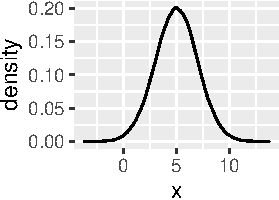
\includegraphics{Lecture-2_files/figure-beamer/unnamed-chunk-1-1} \end{center}

\end{frame}

\begin{frame}[fragile]{Plot the THEORETICAL Normal distribution}
\protect\hypertarget{plot-the-theoretical-normal-distribution}{}

\begin{Shaded}
\begin{Highlighting}[]
\NormalTok{outcomes<-}\KeywordTok{seq}\NormalTok{(}\OperatorTok{-}\DecValTok{5}\NormalTok{,}\DecValTok{15}\NormalTok{, }\DataTypeTok{length.out =} \FloatTok{1e4}\NormalTok{)}
\NormalTok{out_normal <-}\StringTok{ }\KeywordTok{tibble}\NormalTok{(}\DataTypeTok{outcomes =}\NormalTok{ outcomes, }
                     \DataTypeTok{rel_freq =} \KeywordTok{dnorm}\NormalTok{(outcomes, }\DataTypeTok{mean =} \DecValTok{5}\NormalTok{, }\DataTypeTok{sd =} \DecValTok{2}\NormalTok{))}
\KeywordTok{ggplot}\NormalTok{(out_normal, }\KeywordTok{aes}\NormalTok{(}\DataTypeTok{x=}\NormalTok{outcomes,}\DataTypeTok{y =}\NormalTok{ rel_freq))}\OperatorTok{+}
\StringTok{   }\KeywordTok{geom_line}\NormalTok{()}
\end{Highlighting}
\end{Shaded}

\begin{center}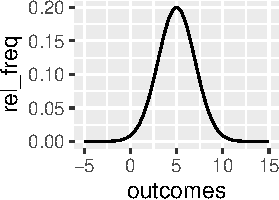
\includegraphics{Lecture-2_files/figure-beamer/unnamed-chunk-2-1} \end{center}

\end{frame}

\begin{frame}{Examples of common distributions in biological research}
\protect\hypertarget{examples-of-common-distributions-in-biological-research-1}{}

\begin{itemize}
\tightlist
\item
  Binomial distribution

  \begin{itemize}
  \tightlist
  \item
    family of distributions
  \item
    Describes potential outcomes: \#successes out of n independent
    trials
  \item
    defined by two parameters:

    \begin{itemize}
    \tightlist
    \item
      n = \# of independent trials
    \item
      p = probability of success in a trial
    \end{itemize}
  \end{itemize}
\end{itemize}

\end{frame}

\begin{frame}[fragile]{Sample from a binomial distribution}
\protect\hypertarget{sample-from-a-binomial-distribution}{}

\begin{Shaded}
\begin{Highlighting}[]
\NormalTok{sample_binomial <-}\StringTok{ }\KeywordTok{tibble}\NormalTok{(}\DataTypeTok{x =} \KeywordTok{rbinom}\NormalTok{(}\FloatTok{1e4}\NormalTok{, }\DataTypeTok{size =} \DecValTok{100}\NormalTok{, }\DataTypeTok{prob =} \FloatTok{0.95}\NormalTok{))}
\KeywordTok{ggplot}\NormalTok{(sample_binomial, }\KeywordTok{aes}\NormalTok{(}\DataTypeTok{x =}\NormalTok{ x))}\OperatorTok{+}
\StringTok{   }\KeywordTok{geom_histogram}\NormalTok{(}\DataTypeTok{binwidth =} \FloatTok{0.5}\NormalTok{)}
\end{Highlighting}
\end{Shaded}

\begin{center}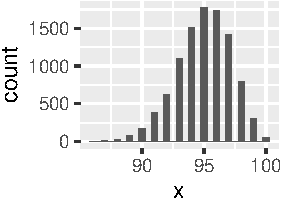
\includegraphics{Lecture-2_files/figure-beamer/unnamed-chunk-3-1} \end{center}

\end{frame}

\begin{frame}[fragile]{Plot the THEORETICAL binomial distribution}
\protect\hypertarget{plot-the-theoretical-binomial-distribution}{}

\begin{Shaded}
\begin{Highlighting}[]
\NormalTok{outcomes<-}\KeywordTok{seq}\NormalTok{(}\DecValTok{71}\NormalTok{,}\DecValTok{100}\NormalTok{, }\DataTypeTok{by=}\DecValTok{1}\NormalTok{)}
\NormalTok{outcomes_binomial <-}\StringTok{ }\KeywordTok{tibble}\NormalTok{(}\DataTypeTok{outcomes =}\NormalTok{ outcomes, }
                            \DataTypeTok{prob =} \KeywordTok{dbinom}\NormalTok{(outcomes, }\DataTypeTok{size=}\DecValTok{100}\NormalTok{, }\DataTypeTok{prob=}\FloatTok{0.95}\NormalTok{))}
\KeywordTok{ggplot}\NormalTok{(outcomes_binomial, }\KeywordTok{aes}\NormalTok{(}\DataTypeTok{x=}\NormalTok{outcomes,}\DataTypeTok{y =}\NormalTok{ prob))}\OperatorTok{+}
\StringTok{   }\KeywordTok{geom_bar}\NormalTok{(}\DataTypeTok{stat=}\StringTok{"identity"}\NormalTok{)}
\end{Highlighting}
\end{Shaded}

\begin{center}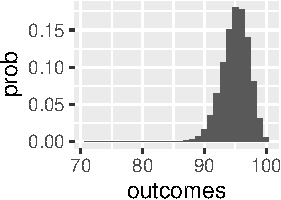
\includegraphics{Lecture-2_files/figure-beamer/unnamed-chunk-4-1} \end{center}

\end{frame}

\begin{frame}{Sampling from a distribution: A data-generating machine}
\protect\hypertarget{sampling-from-a-distribution-a-data-generating-machine}{}

(Graphical description of data generating machine - rnorm) (AR(1)
process)

Now let's look at this from the other end. Using data, can we build a
machine that may have generated our data?

\end{frame}

\begin{frame}[fragile]{Machine 1: Precipitation -\textgreater{} Yield}
\protect\hypertarget{machine-1-precipitation---yield}{}

\begin{Shaded}
\begin{Highlighting}[]
\KeywordTok{set.seed}\NormalTok{(}\DecValTok{202073}\NormalTok{)}
\NormalTok{annual_rain<-}\KeywordTok{seq}\NormalTok{(}\DecValTok{11}\NormalTok{,}\DecValTok{100}\NormalTok{, }\DecValTok{1}\NormalTok{)}
\NormalTok{yield <-}\StringTok{ }\DecValTok{2} \OperatorTok{+}\StringTok{ }\DecValTok{5}\OperatorTok{*}\NormalTok{annual_rain }\OperatorTok{-}\StringTok{ }\FloatTok{0.04}\OperatorTok{*}\StringTok{ }\NormalTok{annual_rain}\OperatorTok{^}\DecValTok{2} \OperatorTok{+}\StringTok{ }\KeywordTok{rnorm}\NormalTok{(}\DecValTok{90}\NormalTok{,}\DecValTok{0}\NormalTok{,}\DecValTok{10}\NormalTok{)}
\NormalTok{yield_dat<-}\KeywordTok{tibble}\NormalTok{(}\DataTypeTok{annual_rain =}\NormalTok{ annual_rain, }\DataTypeTok{yield=}\NormalTok{yield)}
\KeywordTok{ggplot}\NormalTok{(yield_dat, }\KeywordTok{aes}\NormalTok{(annual_rain, yield))}\OperatorTok{+}\KeywordTok{geom_point}\NormalTok{()}
\end{Highlighting}
\end{Shaded}

\begin{center}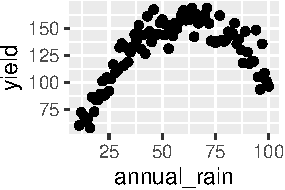
\includegraphics{Lecture-2_files/figure-beamer/unnamed-chunk-5-1} \end{center}

\end{frame}

\begin{frame}[fragile]{Machine 2: Precipitation -\textgreater{} Yield,
AR process}
\protect\hypertarget{machine-2-precipitation---yield-ar-process}{}

\begin{Shaded}
\begin{Highlighting}[]
\KeywordTok{set.seed}\NormalTok{(}\DecValTok{202073}\NormalTok{)}
\NormalTok{annual_rain<-}\StringTok{ }\KeywordTok{rep}\NormalTok{(}\DecValTok{30}\NormalTok{,}\DecValTok{50}\NormalTok{); yield <-}\KeywordTok{rep}\NormalTok{(}\DecValTok{150}\NormalTok{,}\DecValTok{50}\NormalTok{)}
\ControlFlowTok{for}\NormalTok{ (i }\ControlFlowTok{in} \DecValTok{2}\OperatorTok{:}\DecValTok{50}\NormalTok{) \{}
\NormalTok{     annual_rain[i]<-}\StringTok{ }\FloatTok{0.3}\OperatorTok{*}\NormalTok{annual_rain[i}\DecValTok{-1}\NormalTok{] }\OperatorTok{+}\StringTok{ }\KeywordTok{rnorm}\NormalTok{(}\DecValTok{1}\NormalTok{,}\DecValTok{30}\NormalTok{,}\DecValTok{10}\NormalTok{)}
\NormalTok{     yield[i]<-}\StringTok{ }\DecValTok{5}\OperatorTok{*}\NormalTok{annual_rain[i] }\OperatorTok{-}\StringTok{ }\FloatTok{0.04}\OperatorTok{*}\StringTok{ }\NormalTok{annual_rain[i]}\OperatorTok{^}\DecValTok{2} \OperatorTok{+}\StringTok{ }
\StringTok{        }\FloatTok{0.2}\OperatorTok{*}\NormalTok{yield[i}\DecValTok{-1}\NormalTok{] }\OperatorTok{+}\StringTok{ }\KeywordTok{rnorm}\NormalTok{(}\DecValTok{1}\NormalTok{,}\DecValTok{0}\NormalTok{,}\DecValTok{10}\NormalTok{)}
\NormalTok{\}}
\NormalTok{yield_dat2<-}\KeywordTok{tibble}\NormalTok{(}\DataTypeTok{year =} \DecValTok{1951}\OperatorTok{:}\DecValTok{2000}\NormalTok{, }\DataTypeTok{rain =}\NormalTok{ annual_rain, }\DataTypeTok{yield=}\NormalTok{yield)}
\end{Highlighting}
\end{Shaded}

\end{frame}

\begin{frame}[fragile]{Machine 2: Precipitation -\textgreater{} Yield,
AR process}
\protect\hypertarget{machine-2-precipitation---yield-ar-process-1}{}

\begin{block}{Annual rain between 1951 and 2000}

\begin{Shaded}
\begin{Highlighting}[]
\KeywordTok{ggplot}\NormalTok{(yield_dat2, }\KeywordTok{aes}\NormalTok{(year, rain))}\OperatorTok{+}\KeywordTok{geom_line}\NormalTok{()}
\end{Highlighting}
\end{Shaded}

\begin{center}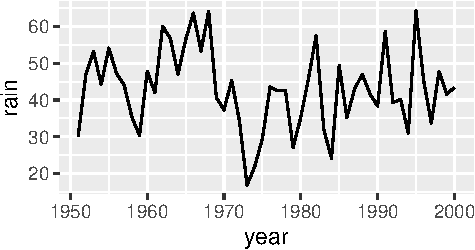
\includegraphics{Lecture-2_files/figure-beamer/unnamed-chunk-7-1} \end{center}

\end{block}

\end{frame}

\begin{frame}[fragile]{Machine 2: Precipitation -\textgreater{} Yield,
AR process}
\protect\hypertarget{machine-2-precipitation---yield-ar-process-2}{}

\begin{block}{Crop yield between 1951 and 2000}

\begin{Shaded}
\begin{Highlighting}[]
\KeywordTok{ggplot}\NormalTok{(yield_dat2, }\KeywordTok{aes}\NormalTok{(year, yield))}\OperatorTok{+}\KeywordTok{geom_line}\NormalTok{()}
\end{Highlighting}
\end{Shaded}

\begin{center}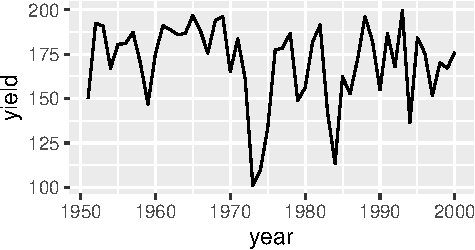
\includegraphics{Lecture-2_files/figure-beamer/unnamed-chunk-8-1} \end{center}

\end{block}

\end{frame}

\begin{frame}[fragile]{Machine 2: Precipitation -\textgreater{} Yield,
AR process}
\protect\hypertarget{machine-2-precipitation---yield-ar-process-3}{}

\begin{block}{Crop yield vs Annual rain}

\begin{Shaded}
\begin{Highlighting}[]
\KeywordTok{ggplot}\NormalTok{(yield_dat2, }\KeywordTok{aes}\NormalTok{(rain, yield))}\OperatorTok{+}\KeywordTok{geom_point}\NormalTok{()}
\end{Highlighting}
\end{Shaded}

\begin{center}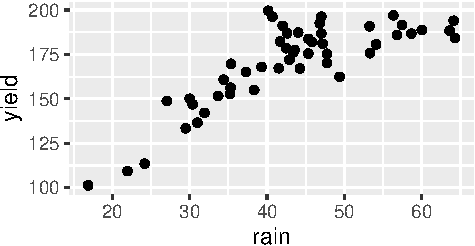
\includegraphics{Lecture-2_files/figure-beamer/unnamed-chunk-9-1} \end{center}

\end{block}

\end{frame}

\begin{frame}{Summary}
\protect\hypertarget{summary}{}

\begin{itemize}
\tightlist
\item
  A probability distribution: a set of possible outcomes and associated
  probabilities
\item
  Data generating process: set of rules for generating set of outcomes
\item
  Probability: from rules to data
\item
  Statistics: from data to rules
\end{itemize}

\begin{block}{Statistics: re-constructing the rules, given the data}

\end{block}

\begin{block}{The Ultimate Challange!}

\end{block}

\end{frame}

\end{document}
